% ---------------------------------------------------------------------
% ---------------------------------------------------------------------
% ---------------------------------------------------------------------

\chapter[Modern techniques for the analysis of metabolomic data]{Modern techniques for the analysis of metabolomic data}
\label{chapter:modern_techniques}


% ---------------------------------------------------------------------
% ---------------------------------------------------------------------
\section{Projection based methods}
\label{projectionmethods}
In the previous chapter, the projection technique known as PCA has been introduced. As explained in section \ref{sec:PCA}, this method works by performing a dimension reduction to an original data matrix with dimensions $I \times J$, to a projected data matrix with dimensions $I \times M$, where $M\leq J$. Each new component of the projected data matrix is built trying to capture as much of the variability from the original data matrix as possible. So PCA is a projection technique that tries to reduce the dimensionality of the data while trying to maximize the information kept from the original data. This approach can be great for performing exploratory analysis of a data set or unsupervised analysis, but can be inefficient for performing supervised analysis such as regression or classification. The reason for this is that, while variables with the highest variability carry most of the information of the original data matrix, they do not necessarily have to be the ones able to explain the response that one is trying to predict \parencite{kettaneh2005pca}. A conceptual explanation of this is presented in \autoref{figura02}.

\begin{figure}[htbp]\centering
		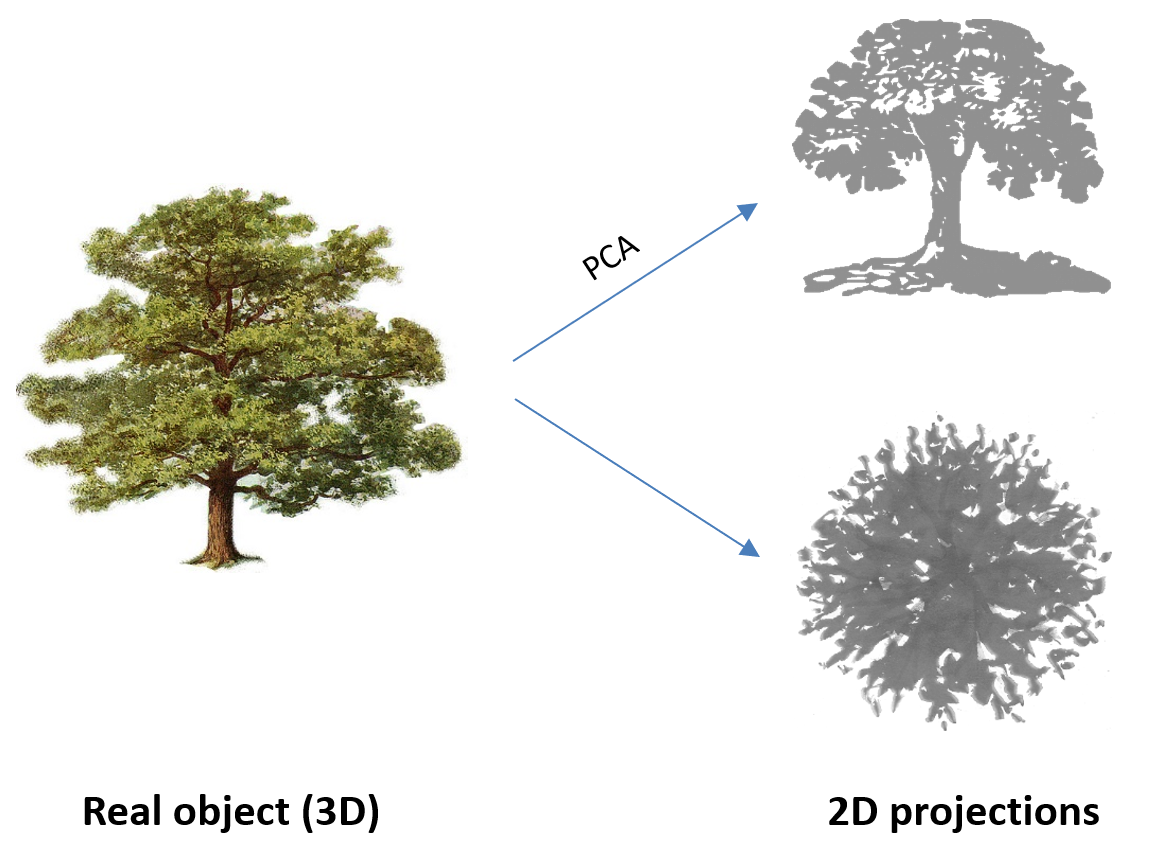
\includegraphics[width=.6\textwidth]{figura02}
		\caption[Differences between PCA and PLS]{Variables with less variability can be the ones related to the response, thus being infrarepresented in the first components of PCA. In this example, if one wanted to predict the amount of shadow dropped by the tree, the PCA projection would not be efficient, while the other presented projection fully captures the target prediction. On the other hand, the PCA projection makes the tree fully recognizable, while the other projection makes it hard to even guess there is a tree.}
		\label{figura02}
	\end{figure}

Thus, if the aim is prediction, projection for maximizing the explained variability on the original data matrix is not the best approach. It is much better to maximize covariance with the response. This is how the technique Partial Least Squares (PLS) works.

\subsection{Partial Least Squares}
In linear regression, there is a limit on the number of variables that can enter a model for a specific sample size. Recent studies have shown that a minimum of two independent observations per variable are needed for estimating regression coefficients with reasonable bias \parencite{austin2015number}. Metabolomic data sets usually have many more variables than observations, so linear regression models are not a viable alternative for analyzing these data sets. Linear regression also suffers from multicollinearity, so when highly correlated predictors are used together in a model their coefficients get unstable and standard errors grow wildly \parencite{alin2010multicollinearity}. PLS can be seen as an extension of multiple linear regression designed to overcome the mentioned drawbacks. It can analyze data sets with strongly correlated variables and handle situations where the number of variables far exceeds the number of observations \parencite{wold2001pls}. Additionally, PLS can also simultaneously model several response variables. It is important to note that results of PLS (and of projection methods in general) depend on the scaling of the data so, before the analyses, pre-processing of the \textbf{X} and \textbf{Y} variables should be considered.
A scheme of the PLS model is depicted in \autoref{figura17}.

\begin{figure}[hbtp]
	\centering
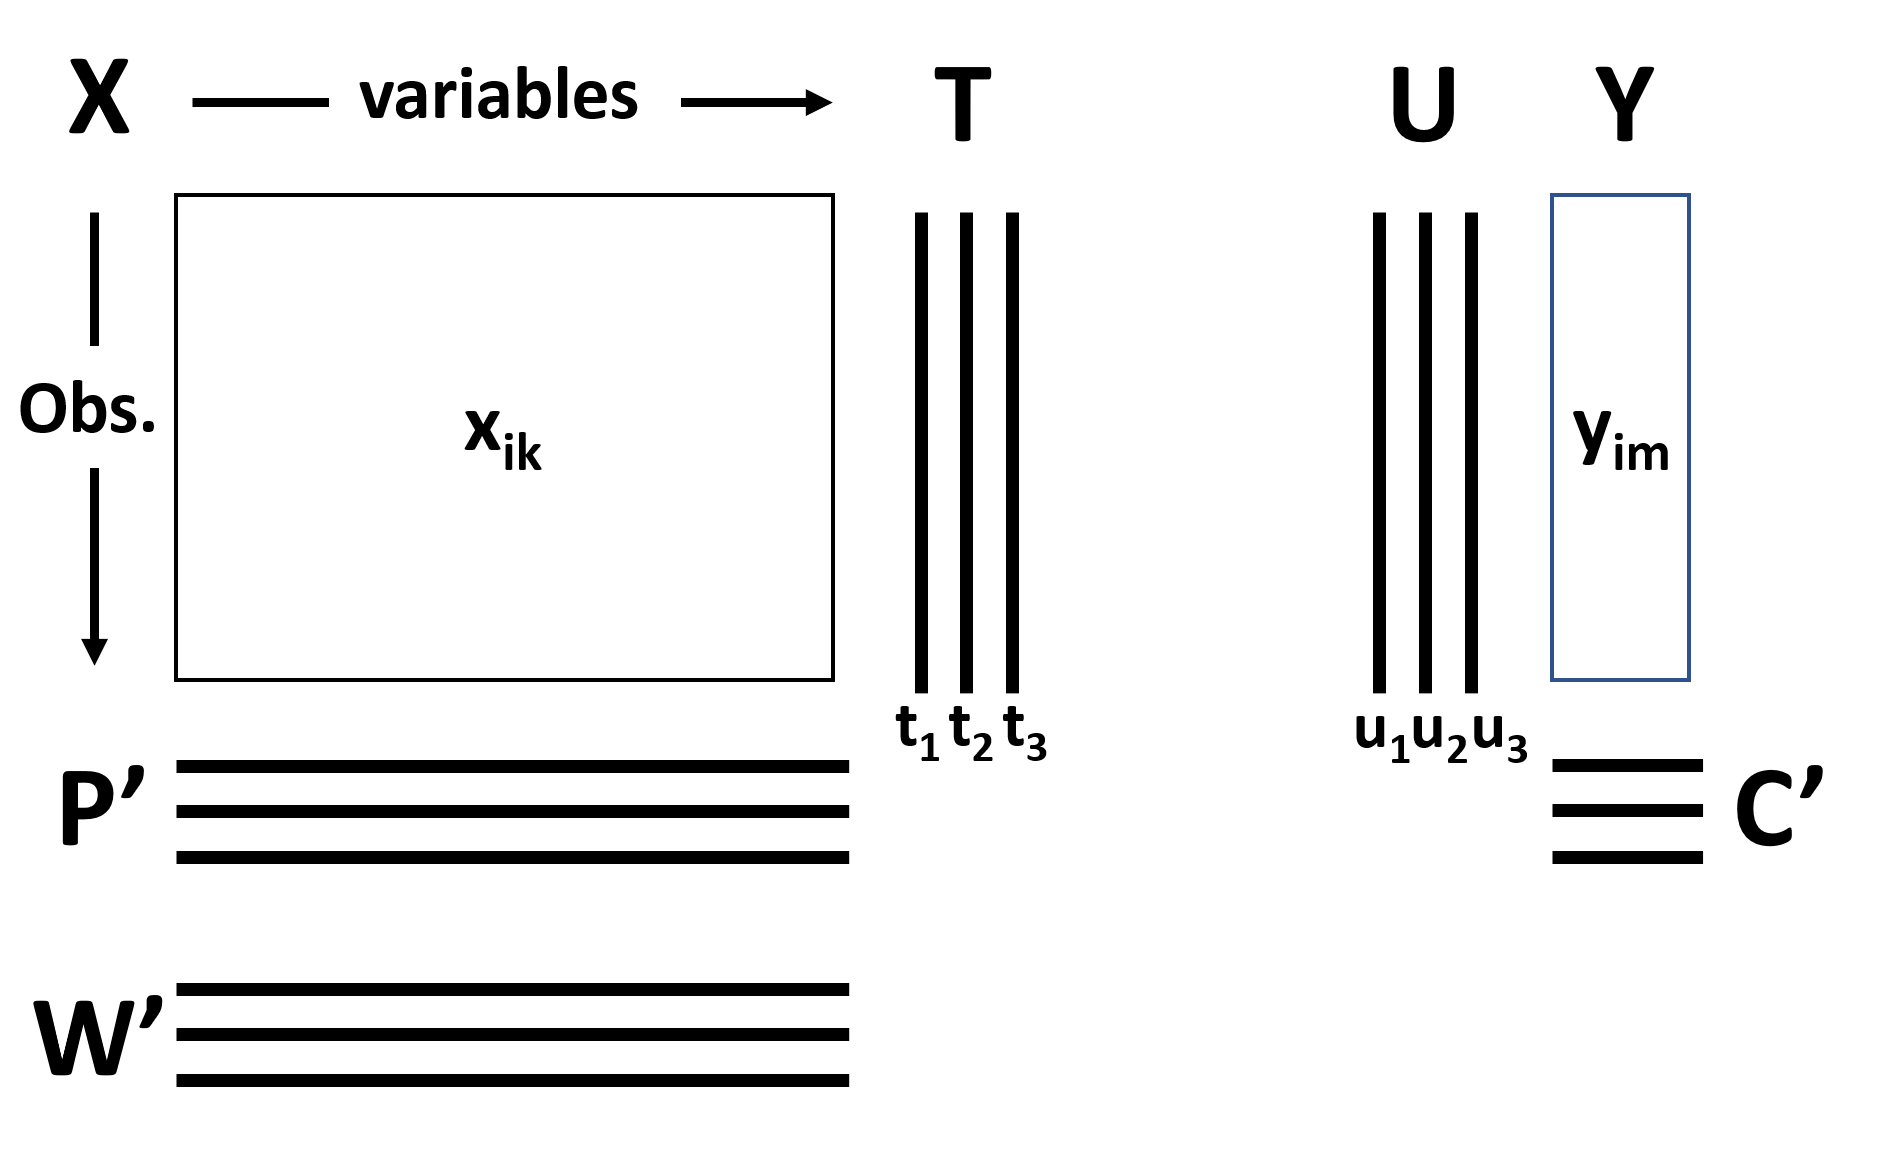
\includegraphics[width=0.7\textwidth]{figura17.png}
\caption[Scheme of the PLS model]{Scheme of the PLS model \parencite{wold2001pls}. \textbf{X} is the matrix of predictors and \textbf{Y} is the matrix of responses. Additional matrices are generated at the different modelling steps.}
\label{figura17}
\end{figure}

The PLS model finds latent variables (denoted by $\text{t}_a$, where a = 1, 2, \dots, A) that are predictors of \textbf{Y} (with dimensions $I \times M$) and also model \textbf{X} (with dimensions $I \times K$), by maximizing the covariance between their latent structures. These latent variables are also called X-scores and are orthogonal. They are estimated as linear combinations of the original variables using different weights denoted by $\text{w}^*_{ka}$ (\autoref{equation08}). 

\begin{equation}
\label{equation08}
\textbf{\text{T}}=\textbf{\text{XW}}^*
\end{equation}

X-scores are multiplied by the loadings $\text{p}_{ak}$ in order to obtain the residuals in \textbf{X}, denoted as \textbf{E} (\autoref{equation09}).

\begin{equation}
\label{equation09}
\textbf{\text{X}}=\textbf{\text{TP}}'+\textbf{\text{E}}
\end{equation}

Analogously, the Y-scores are multiplied by the weights (denoted by $\text{c}_{am}$) minimizing residuals in \textbf{Y}, denoted as \textbf{G} (\autoref{equation10}).

\begin{equation}
\label{equation10}
\textbf{\text{Y}}=\textbf{\text{UC}}'+\textbf{\text{G}}
\end{equation}

As stated before, X-scores are good predictors of \textbf{Y} (\autoref{equation11}).

\begin{equation}
\label{equation11}
\textbf{\text{Y}}=\textbf{\text{TC}}'+\textbf{\text{F}}
\end{equation}

Where \textbf{F} is the residuals matrix from \textbf{Y}. Alternatively, \autoref{equation11} can be rewritten as follows (\autoref{equation12}):

\begin{equation}
\label{equation12}
\textbf{\text{Y}}=\textbf{\text{XW}}^*\textbf{\text{C}}'+\textbf{\text{F}}=\textbf{\text{XB}}+\textbf{\text{F}}
\end{equation}

Which resembles a multiple linear regression model where the predictors matrix \textbf{X} is multiplied by the coefficients matrix \textbf{B} to predict \textbf{Y}.

PLS is, consequently, a modelling technique able to effectively deal with metabolomic data. Correlated variables and data sets with many more variables than observations can be properly analyzed and results are easily interpreted with the help of useful plots of the scores, weights and predictions of the model (\autoref{figura18}).

\begin{figure}[hbtp]
	\centering
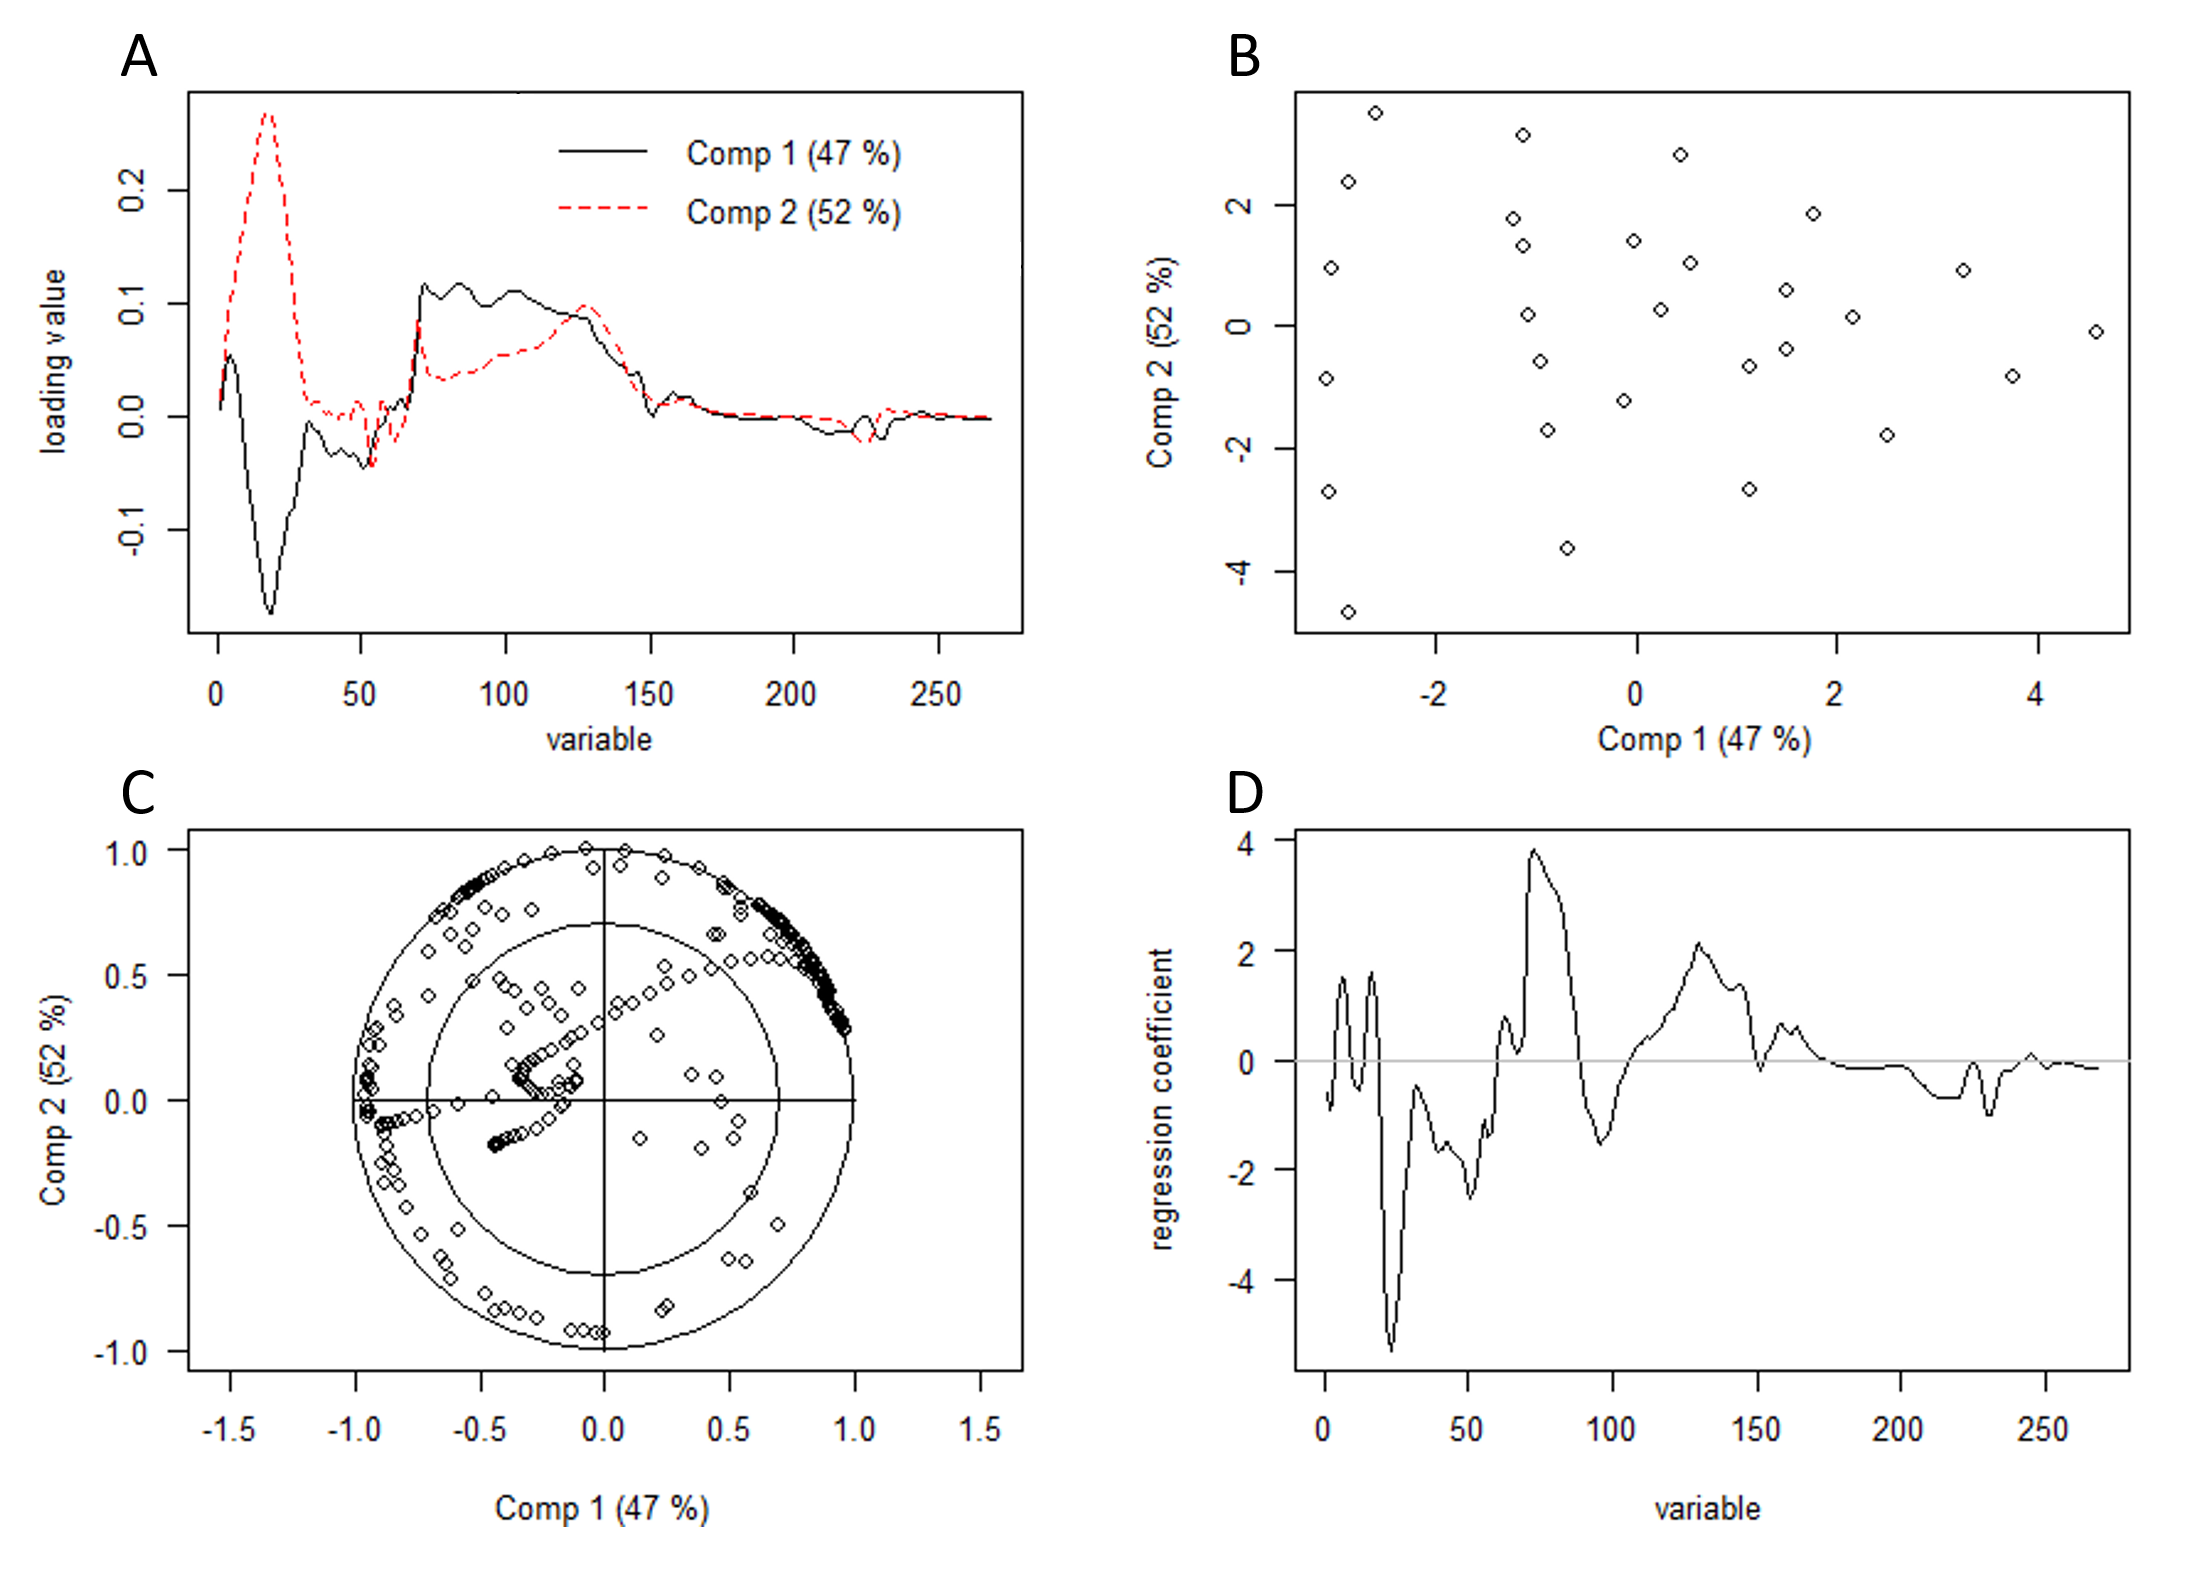
\includegraphics[width=0.82\textwidth]{figura18.png}
\caption[Plots of a PLS model]{Plots of a PLS model. \textbf{A} shows the weights for each variable in the two first components. \textbf{B} shows the scores for each observation in the first two components. \textbf{C} represents the correlations between each variable and the first two components.  \textbf{D} shows the regression coefficients of the model.}
\label{figura18}
\end{figure}


\section{Penalization methods}
\label{penalmethods}
Another set of techniques able to manage metabolomic data sets are the penalization methods. These methods are motivated by the relationship between model complexity and prediction error, also known as bias-variance trade-off \parencite{hastie2001model}. As depicted in \autoref{figura19}, prediction error in the same data set used to fit a specific model always decreases when increasing the complexity of the model. On the other hand, prediction error in new data decreases at first, reaching a minimum at a specific model complexity, and increases later again as model complexity keeps growing larger.

\begin{figure}[hbtp]
	\centering
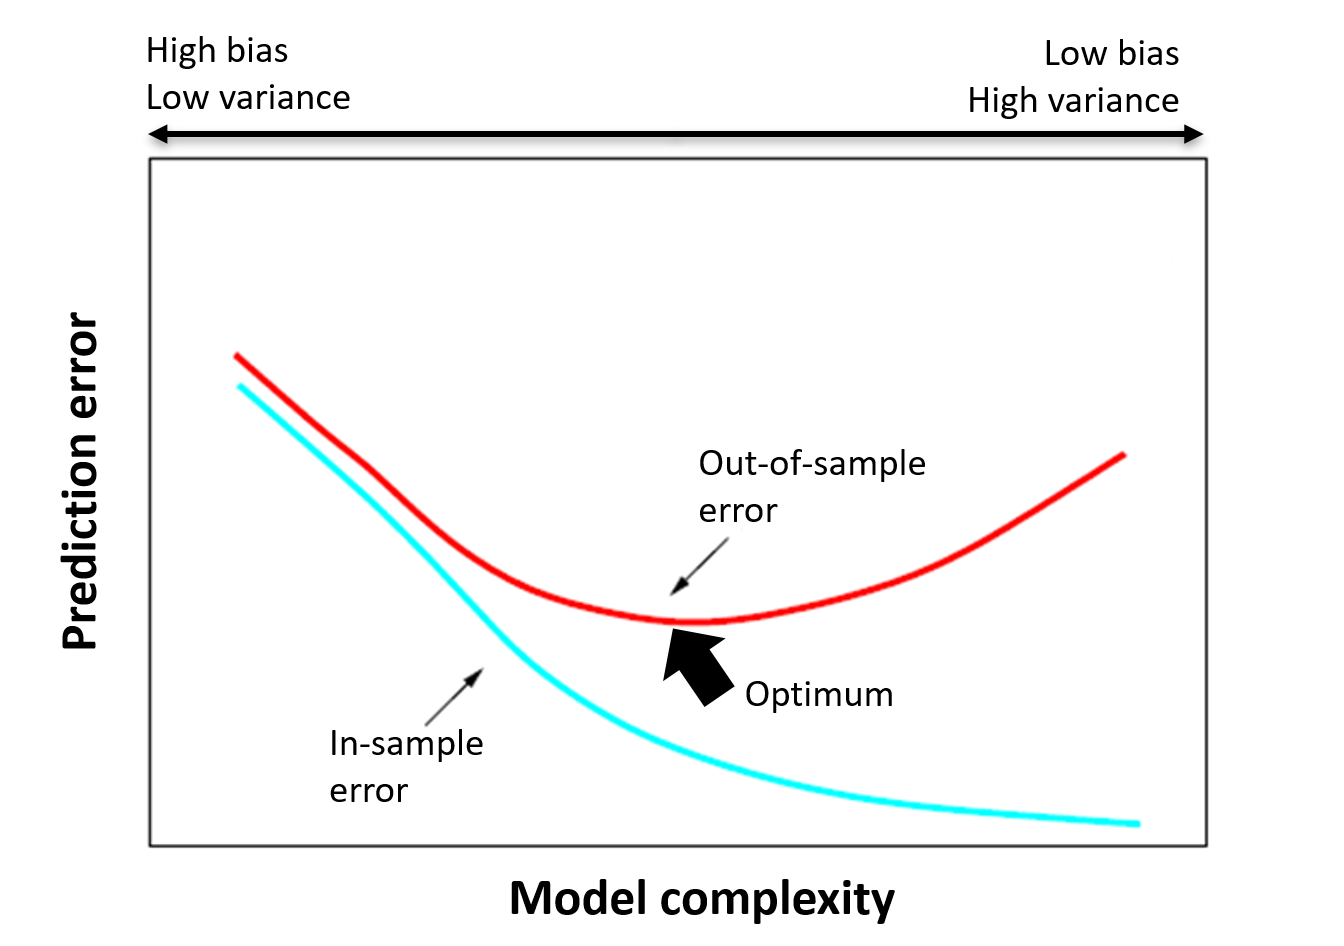
\includegraphics[width=0.75\textwidth]{figura19.png}
\caption{Behavior of prediction error in training (in-sample) and test (out-of-sample) data.}
\label{figura19}
\end{figure}

As previously described, metabolomic data sets are characterized by having a large number of variables and relatively a low number of observations. Trying to fit a model with all the variables in this situation would correspond to the extreme right side of the plot in \autoref{figura19} with low bias and high variance. This is the reason why multiple regression models cannot be fit to these data, variance grows to infinite as the number of predictor variables increases in the model. But this relationship between bias-variance and model complexity gives us the key for improving the standard linear models: increasing bias will reduce the variance, potentially obtaining a lower out-of-sample prediction error because model complexity has been decreased. Thus, the solution for being able to fit linear models to metabolomic data is to bias them. The full reasoning behind this last sentence can be better understood with the explanation provided in \autoref{figura20}.

\begin{figure}[hbtp]
	\centering
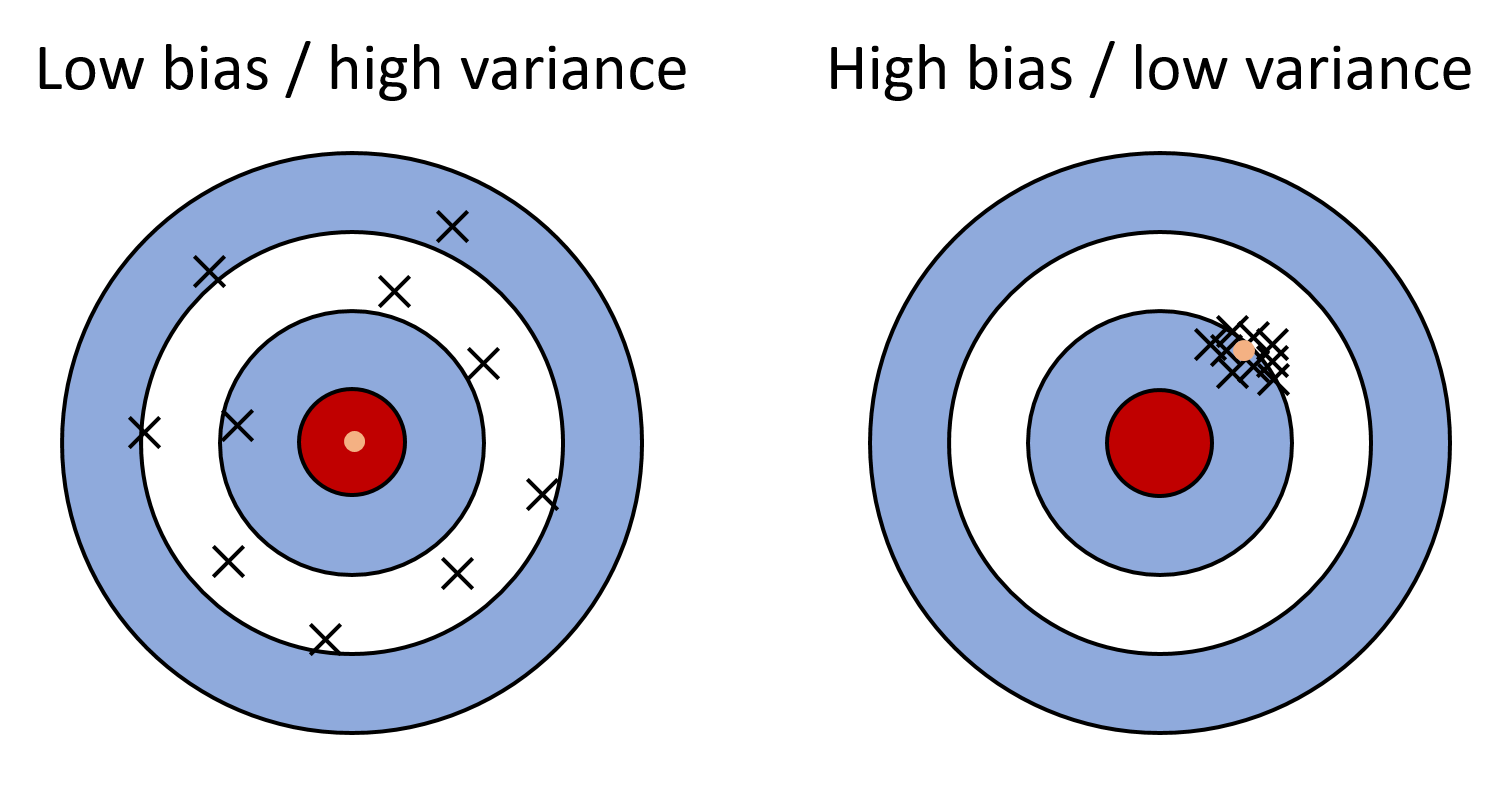
\includegraphics[width=0.75\textwidth]{figura20.png}
\caption[No bias / high variance vs. Bias / low variance situation]{In both targets each black cross represents an estimation of a specific model to different samples of the same population and the orange dot represents the average estimation of all of them. In the left target there is no bias, with the orange dot right at the bullseye, but estimation from the different samples are wildly spread with a very high variability. In the right target, there is a perceptible amount of bias, the orange dot lies out of the bullseye, but all estimations from the different samples are concentrated in a small area around the average estimation. Usually, only one sample (one data set) is available for performing the estimation, so the advantage of introducing bias to lower variance is evident.}
\label{figura20}
\end{figure}

\subsection{Ridge regression}
The first developed penalization method for linear regression was ridge regression \parencite{hoerl1970ridge}. This method consists in solving the ordinary least squares problem, but introduces a restriction to the solution. This restriction consists in setting an upper bound on the sum of the squared coefficients (L2 norm) (\autoref{equation13}).

\begin{equation}
\label{equation13}
\begin{split}
\hat{\beta}^{ridge}=\argmin_\beta \sum\limits_{i=1}^N (y_{i}-\beta_{0}-\sum\limits_{j=1}^p x_{ij}\beta_{j})^{2} \\
\textrm{Subject to the restriction:}  \sum\limits_{j=1}^p \beta_{j}^2\leq s
\end{split}
\end{equation}

The inclusion of this restriction to the ordinary least squares problem imposes a reduction in the value of the coefficients, thus biasing their estimation and producing a reduction in the complexity of the model. A graphical explanation of the functioning of the method is represented in \autoref{figura21}.

\begin{figure}[hbtp]
\centering
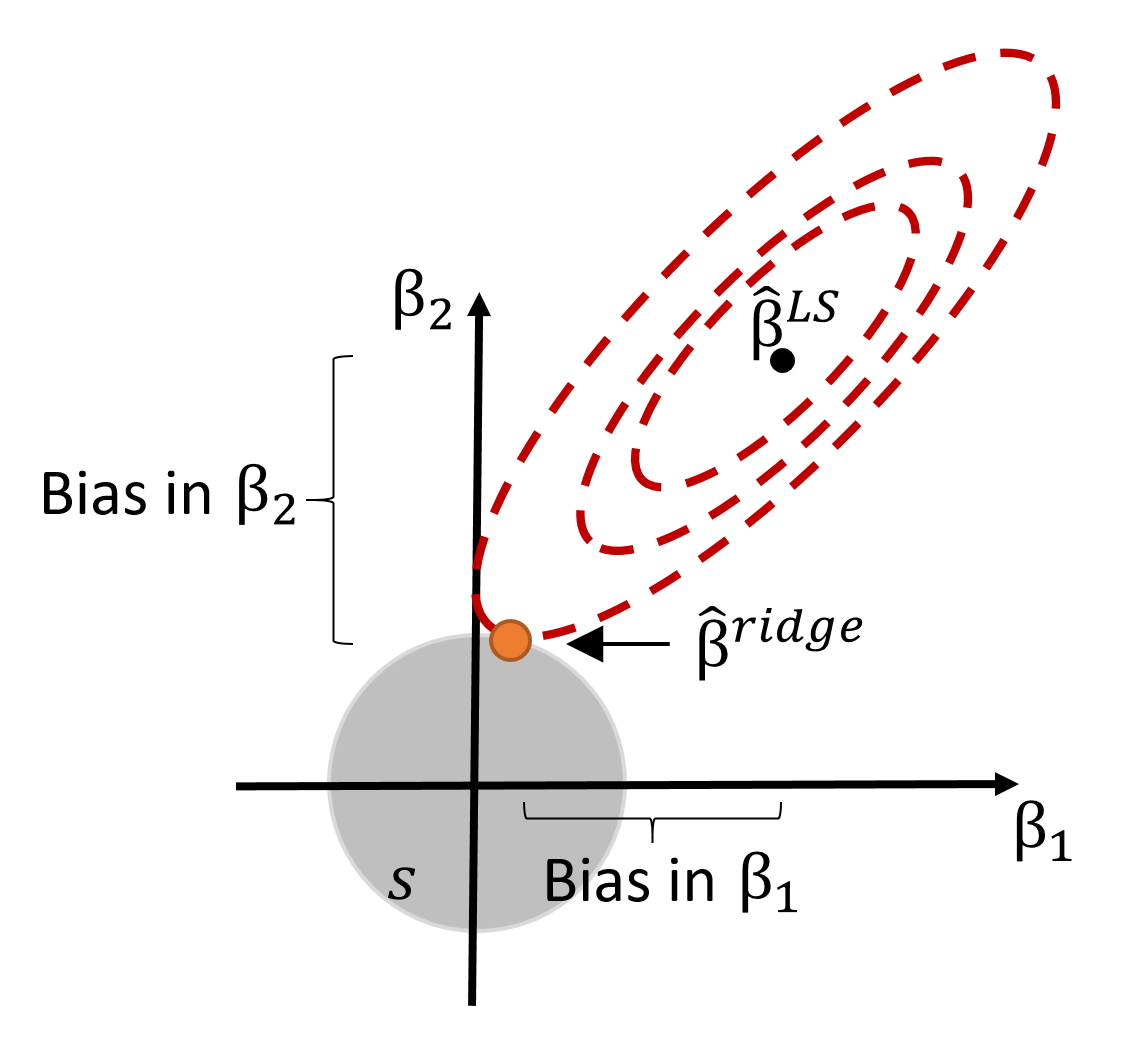
\includegraphics[width=0.6\textwidth]{figura21.png}
\caption[Ridge regression for a linear model with two predictors]{Ridge regression for a linear model with two predictors. As the restriction is intensified (lower value of $s$), the estimation of the coefficients is more biased to zero. Dashed red lines represent least squares contour lines. Grayed area represents the restriction imposed by $s$.}
\label{figura21}
\end{figure}

The solution offered by ridge regression is very similar to that obtained by PLS. A regression model suitable for metabolomic data sets with many, highly correlated variables. Both methods use all the variables for adjusting the model and both models shrink the estimates of the coefficients \parencite{de1995pls}, thus reducing model complexity and therefore variance at a cost of increasing bias.

\subsection{Lasso}
\label{lasso}
In many studies there is the need or interest of not only fitting a predictive model, but also selecting the most important predictors among all the variables present in the data. As it has been exposed in the previous sections, neither PLS nor ridge regression provide a direct method for variable selection. They both use all the variables in the data set for adjusting the model. It is true that there are some post-model-fitting methods for assessing variable importance in the case of PLS \parencite{mehmood2012review}, but they require and additional filtering step after the model has been fitted and are not inherent to the PLS model. The method known as lasso is similar to ridge regression. But instead of setting a bound on the sum of the squared coefficients, it is set on the sum of the absolute values of the coefficients (L1 norm) as seen in \autoref{equation14} \parencite{tibshirani1996regression}. This change in the method of penalization of the coefficients allows that some of them are set to zero when the model is adjusted, thus producing a variable selection at the model-fitting step.

\begin{equation}
\label{equation14}
\begin{split}
\hat{\beta}^{lasso}=\argmin_\beta \sum\limits_{i=1}^N (y_{i}-\beta_{0}-\sum\limits_{j=1}^p x_{ij}\beta_{j})^{2} \\
\textrm{Subject to the restriction:}  \sum\limits_{j=1}^p |\beta_{j}|\leq s
\end{split}
\end{equation}

\vspace{10pt}

\begin{figure}[hbtp]
\centering
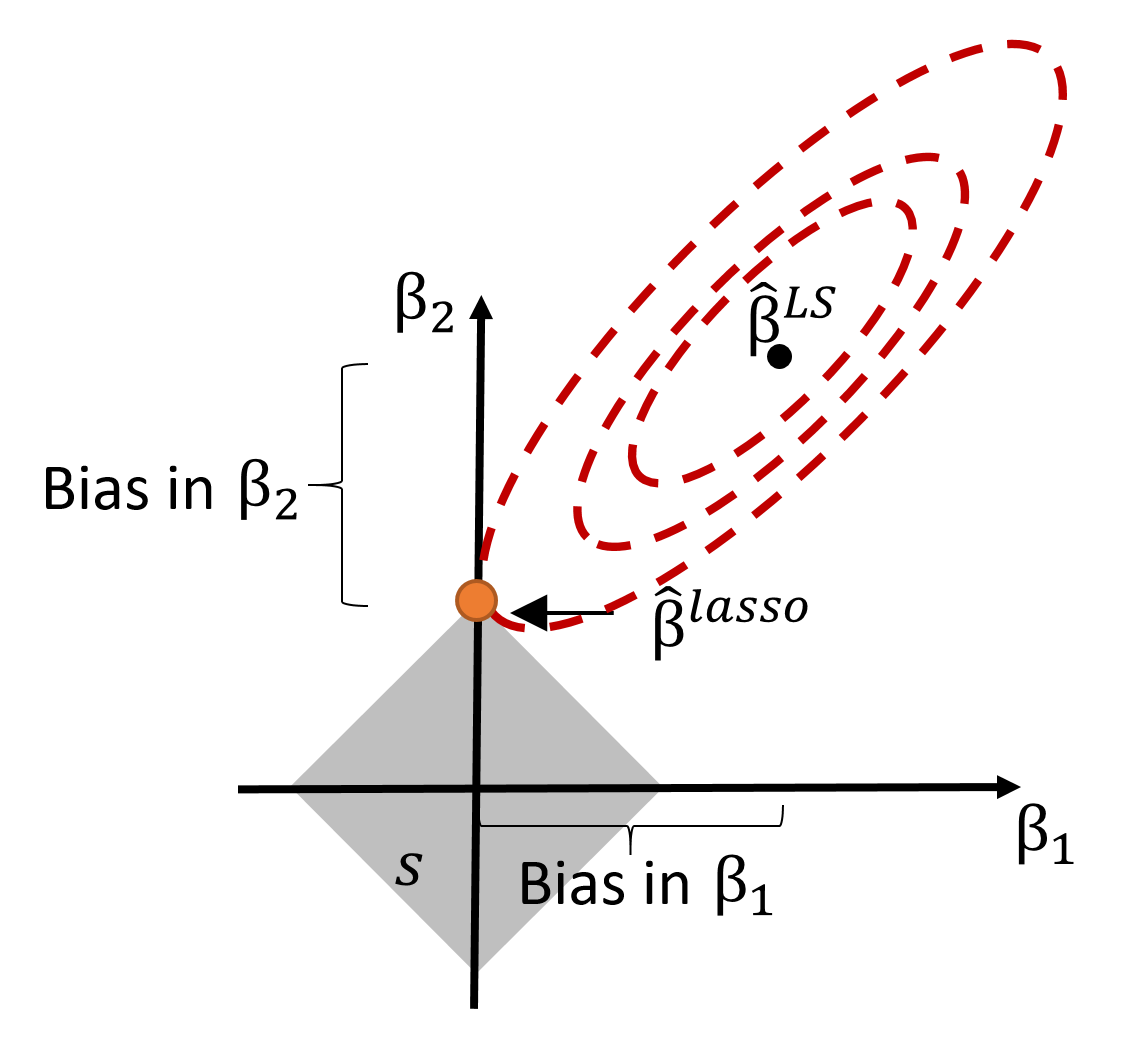
\includegraphics[width=0.6\textwidth]{figura22.png}
\caption[Lasso regression for a linear model with two predictors]{Lasso regression for a linear model with two predictors. As the restriction is intensified (lower value of $s$), the estimation of the coefficients is more biased to zero. Since it is more easier to land in a vertex than in an edge, reducing $s$ forces one of the coefficients to zero. Dashed red lines represent least squares contour lines. Grayed area represents the restriction imposed by $s$.}
\label{figura22}
\end{figure}

\autoref{figura22} shows how increasing the penalization by reducing $s$ forces the parameters to zero, producing a simpler model by deselecting some features. Thus, assuming data are standardized (i.e., mean centered and scaled to unit variance), Lasso automatically selects the most relevant features and discards the others.

The fact that lasso allows for variable selection makes it a very appealing solution for modelling 'omic' data. Unfortunately, unlike PLS and ridge regression, lasso is not able to deal with multicollinearity in an optimal manner \parencite{chong2005performance}, which is a prominent characteristic of metabolimic data. When two (or more) variables are highly correlated, lasso will select one of them discarding the others and, potentially, losing predictive performance and important variables.

\subsection{Elastic net}
Two different penalization methods have been presented, each one with its own benefits and drawbacks. Ridge is able to deal with multicollinearity but does not perform variable selection and lasso performs variable selection but does not deal adequately with multicollinearity. The elastic net algorithm  (EN) was developed in order to merge the good qualities of ridge and elastic net and overcome their limitations \parencite{zou2005regularization}. EN is a flexible combination of the two constrains defined for ridge and lasso. The L1 penalty provides variable selection and the L2 penalty provides stability in the selection of correlated variables. The balance between both penalties is defined by the parameter $\alpha$  (\autoref{equation15}). When $\alpha=0$, elastic net is equivalent to ridge regression, since the L1 constraint is set to zero. On the other hand, when $\alpha=1$, elastic net is equivalent to lasso, since the L2 constraint is set to zero. Values between $\alpha = 0$ and $\alpha = 1$ provide different balances between L1 (more variable selection) and L2 (better handling of multicollinearity) penalizations.

\vspace{10pt}

\begin{equation}
\label{equation15}
\begin{split}
\hat{\beta}^{elastic net}=\argmin_\beta \sum\limits_{i=1}^N (y_{i}-\beta_{0}-\sum\limits_{j=1}^p x_{ij}\beta_{j})^{2} \\
\textrm{Subject to the restriction: }  \alpha \sum\limits_{j=1}^p |\beta_{j}| + (1-\alpha) \sum\limits_{j=1}^p \beta_{j}^2 \leq s
\end{split}
\end{equation}

\vspace{10pt}

\autoref{figura23} depicts the elastic net in a two-variable case and shows how, while keeping the vertices present in lasso, the edges are convex and allow for grouped selection of correlated variables. This is a very attractive solution for the modelling of metabolomic data sets and has been used widely during the last years \parencite{lankinen2010dietary, bowling2014analyzing, liu2015high, ferrario2016mortality}. The only drawback of elastic net compared to lasso and ridge is the inclusion of another parameter in the model. Instead of optimizing only for the value of $s$, elastic net models have also to optimize for the value of $\alpha$, thus requiring more tuning for an appropriate fitting of the data. 

Penalization methods have been used by the author of this thesis for the analysis of different 'omic' data sets with very positive results \parencite{yanez2015two, gonzalez2017prognostic, 10.1371/journal.pone.0202926}.

\begin{figure}[hbtp]
\centering
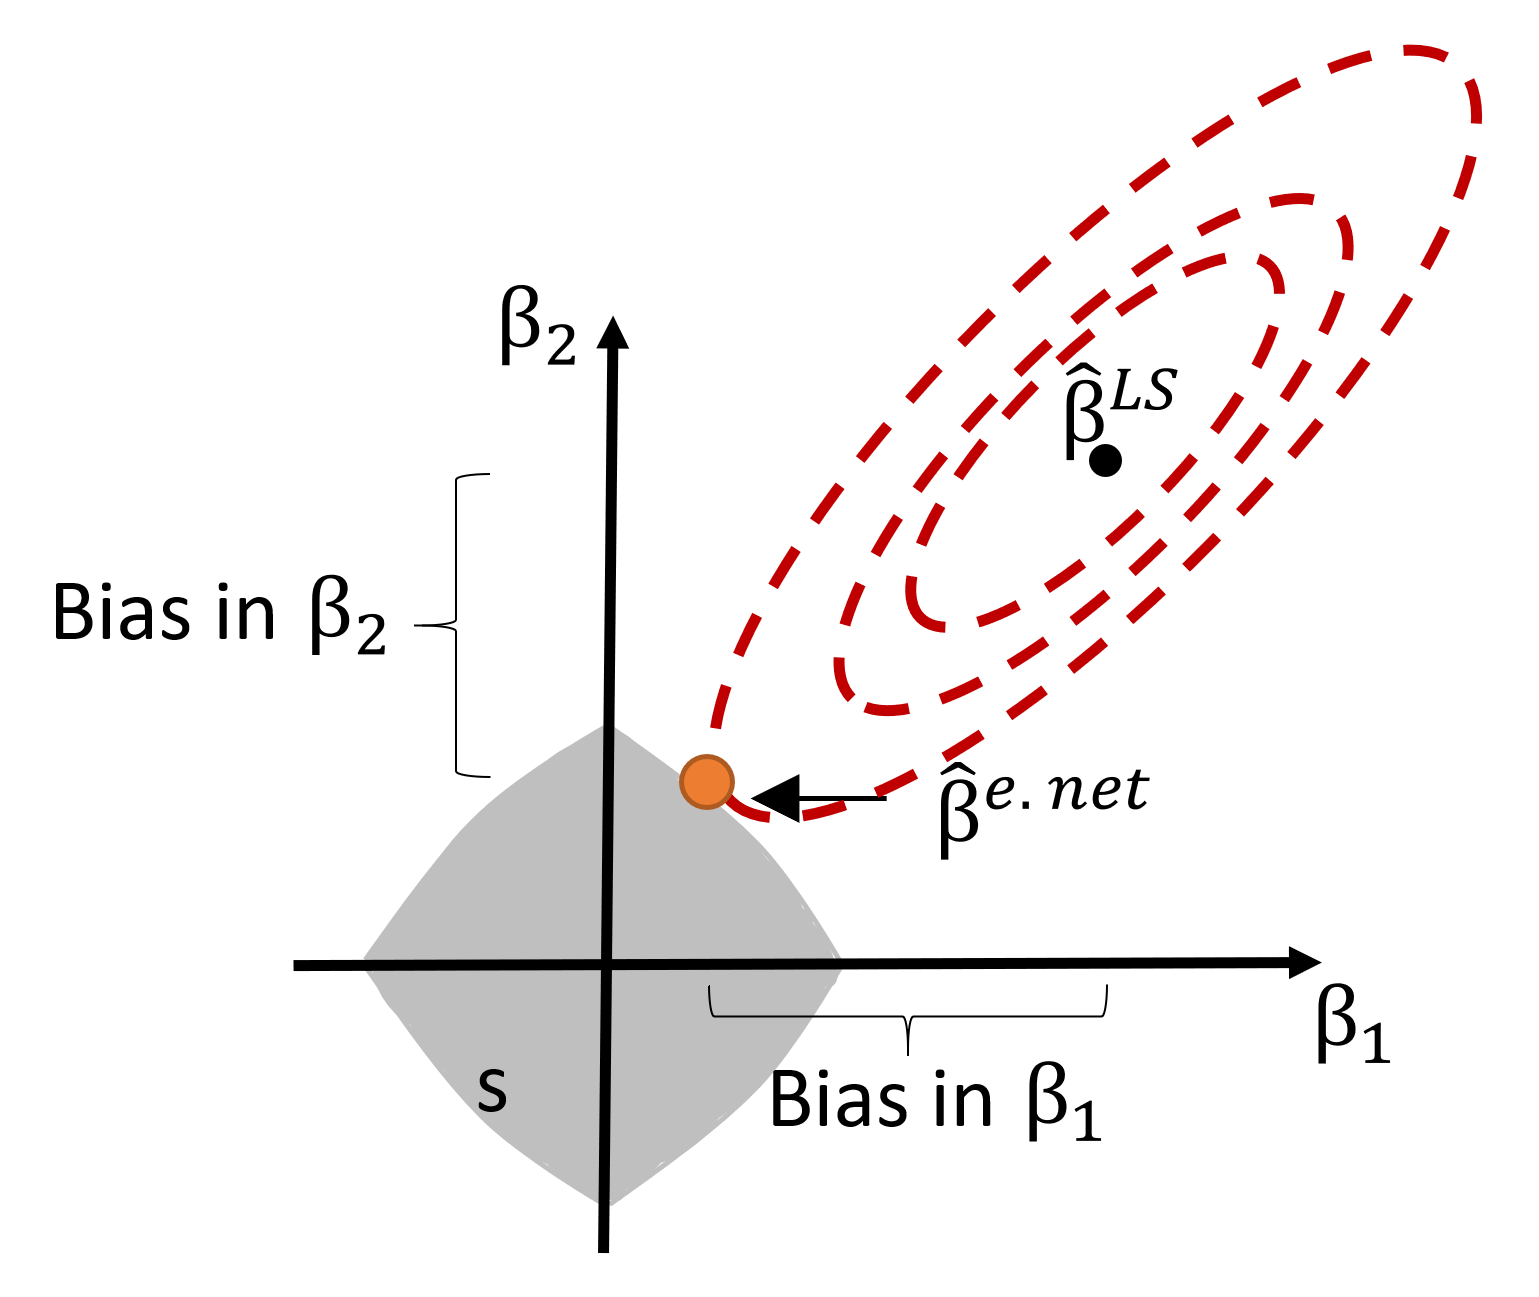
\includegraphics[width=0.6\textwidth]{figura23.png}
\caption[Elastic net regression for a linear model with two predictors]{Elastic net regression for a linear model with two predictors. As the restriction is intensified (lower value of $s$), the estimation of the coefficients is more biased to zero. As in lasso, it is more easier to land in a vertex than in an edge, so many coefficients can be potentially set to zero. But, as in ridge, edges are convex, so highly correlated variables will be selected together. Dashed red lines represent least squares contour lines. Grayed area represents the restriction imposed by $s$.}
\label{figura23}
\end{figure}

\section{Other methods}
Projection based methods and penalization methods are extensions of the standard linear model and can also be extended to generalized linear models and survival models without much effort \parencite{nygaard2008partial, simon2011regularization}. But there are other methods worth mentioning when thinking about dealing with metabolomic data sets. Among them stand out neural networks \parencite{dayhoff2001artificial}, which are highly parametrized models inspired by the functioning of the human brain, support vector machines \parencite{mahadevan2008analysis} based on kernel methods, bayesian networks \parencite{bartel2013statistical} and tree based methods such as regression and classification trees \parencite{venables2002tree, loh2014fifty}, \autoref{figura25}, random forests \parencite{breiman2001random} based on bootstrap resampling \parencite{efron1994introduction} of classification trees and boosting \parencite{freund1996experiments, auret2011empirical}.

\begin{figure}[hbtp]
\centering
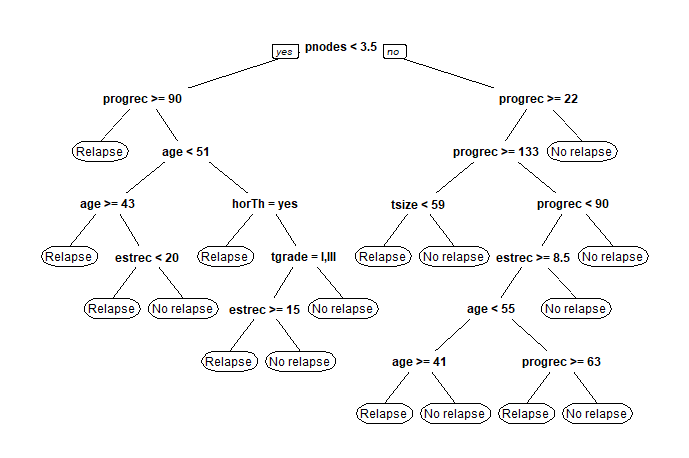
\includegraphics[width=1\textwidth]{figura25.png}
\caption[Classification tree for predicting relapse in breast cancer patients]{Classification tree for predicting relapse in breast cancer patients. Starting from the top one, each node tests a boolean condition which determines the direction of the next node to test until a terminal node is reached and a prediction is made.}
\label{figura25}
\end{figure}
